\chapter{Синхронизација календара за \textit{оwnCloud} платформу}
\label{chap:ownCloudCalendarSynchronization}

У претходним поглављима описани су основни концепти технологија и окружења који су коришћени у развоју датог пројекта, са циљем да се читаоцу омогући да формира слику комплетног, заокруженог, решења. Сам пројекат, који је тема овог рада, може се посматрати као део тог решења. У овом поглављу фокус ће бити постављен на појашњења неких делова његове имплементације.

\section{Жељене функционалности}

Актуелна, званична, верзија \textit{оwnCloud} десктоп клијента обезбеђује само синхронизацију докумената који се налазе на \textit{оwnCloud} платформи. Основни циљ овог пројекта јесте да се развије решење, у виду мултиплатформског десктоп клијента, које би омогућило преузимање информација о креираним догађајима на \textit{оwnCloud} календару и приказ одговарајућих обавештења. Апликација има следећи скуп функционалности:
\begin{itemize}
	\item{синхронизација догађаја на захтев},
	\item{аутоматска синхронизација догађаја},
	\item{могућност управљања аутоматском синхронизацијом (потребна/није потребна, дефинисање временског интервала након којег ће се стартовати,...)},
	\item{преглед преузетих догађаја},
	\item{приступ делу за администрацију догађаја на веб порталу \textit{оwnCloud} платформе},
	\item{приказ одговарајућег обавештења, непосредно пре почетка неког догађаја}.	
\end{itemize}

Ток активности које треба да обезбеде ове функционалности описан је на дијаграму \ref{fig:application_alogorithm}.

\begin{figure}[H]
	\centering
	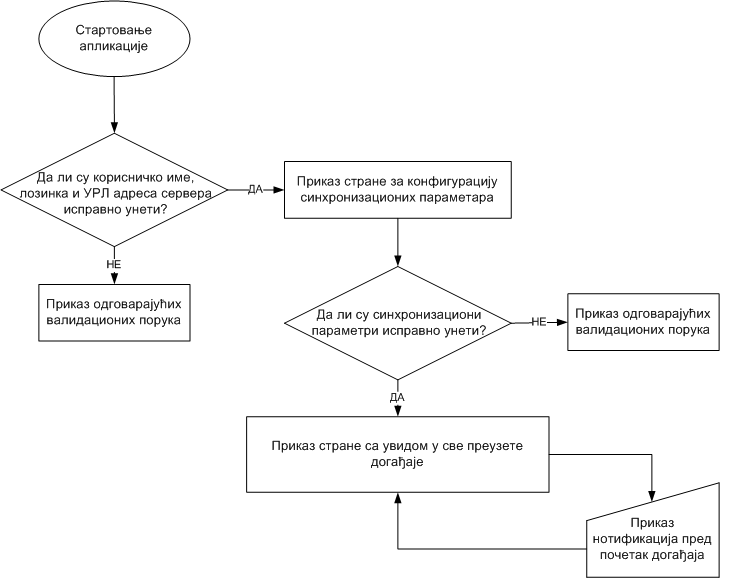
\includegraphics[scale=0.5]{slike/tok_aktivnosti.png}
	\caption{Дијаграм тока активности}
	\label{fig:application_alogorithm}
\end{figure}

На основу приказаног алгоритма  може се стећи јасна и потпуна слика о начину рада саме апликације. У наставку ће бити детаљније објашњене неке интересантније функционалности и биће приказани делови програмског кода, док се комплетан код пројекта може погледати на одговарајућем репозиторијуму\cite{svn_repo}.

\subsection{Аутентификација}

Аутентификација корисника на веб портал \textit{оwnCloud} платформе одрађена је коришћењем класа \textit{WebClient}, \textit{NetworkCredential} које су саставни део \textit{.NET Framework-a}.  Подаци унети на форми за пријаву на систем (Слика \ref{fig:login_form}), која се приказује након стартовања апликације, се прослеђују на верификацију:

\begin{figure}[H]
	\centering
	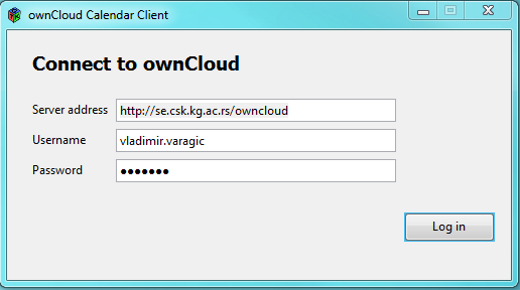
\includegraphics[scale=0.5]{slike/logInForm.png}
	\caption{Форма за пријаву на систем}
	\label{fig:login_form}
\end{figure}

Сви подаци на форми за пријаву су обавезни, па се у случају да неки податак није унет, прикаже одговарајући индикатор:

\begin{figure}[H]
	\centering
	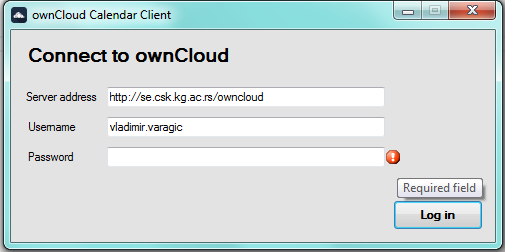
\includegraphics[scale=0.5]{slike/LogInFormReqiredFields.png}
	\caption{Форма за пријаву на систем}
	\label{fig:login_form_required}
\end{figure}

Такође, у случају да неки од података који се уносе приликом пријаве на апликацију (адреса сервера, корисничко име или лозинка) није исправан приказује се одговарајућа порука:

\begin{figure}[H]
	\centering
	\includegraphics[scale=0.5]{slike/logInFailed.png}
	\caption{Форма за пријаву на систем}
	\label{fig:login_form_failed}
\end{figure}

У супротном, ако су сви подаци исправни, корисник успешно приступа апликацији и приказује му се форма за синхронизацију догађаја са \textit{оwnCloud} календара.

\subsection{Синхронизација догађаја на захтев}

Као што је већ наведено у поглављу \textit{5.1.1 Аутентификација}, након успешног приступа апликацији кориснику се приказује форма за конфигурацију синхронизације:

\begin{figure}[H]
	\centering
	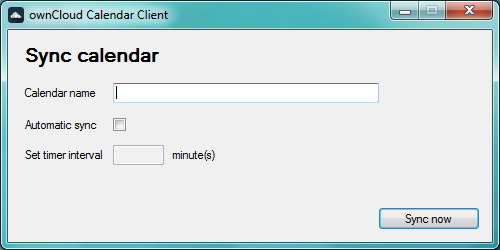
\includegraphics[scale=0.5]{slike/SyncCalendar.png}
	\caption{Синхронизација догађаја са \textit{оwnCloud} календара}
	\label{fig:sync_calendar}
\end{figure}

\textit{OwnCloud} платформа омогућава кориснику да на порталу води више различитих календара тј. да календар дели у различите категорије. 

\begin{figure}[H]
	\centering
	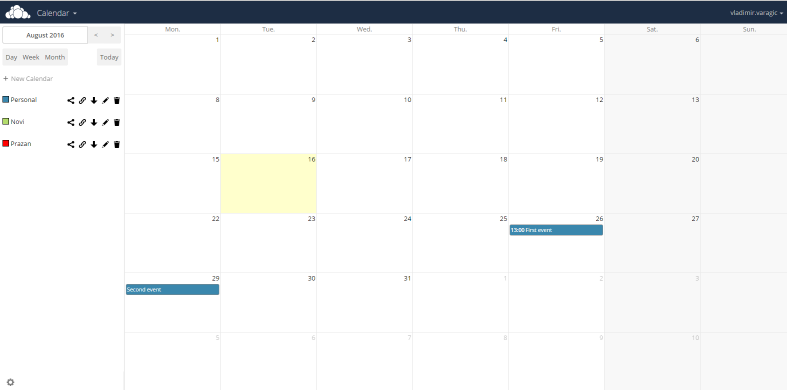
\includegraphics[scale=0.5]{slike/ownCloudCalendar.png}
	\caption{\textit{OwnCloud} календар}
	\label{fig:own_cloud_calendar}
\end{figure}

Са друге стране, синхронизацијом се у једном тренутку могу преузети само догађаји који су везани за једну категорију, тако да је назив календара обавезан податак приликом синхронизације. Такође, приликом покретања синхронизације ради се валидација исправности назива календара и уколико не постоји календар са унетим називом кориснику се прикаже одговарајућа порука. У супротном, ако је унет исправан назив календара, кориснику се приказују догађаји који постоје на наведеном календару. Сам приказ података о догађају биће детаљно описан у секцији \textit{5.1.4 Преглед перузетих догађаја}.

Методе којима се синхронизују подаци приказани су на слици \ref{fig:sync_calendar_method}

\begin{figure}[H]
	\centering
	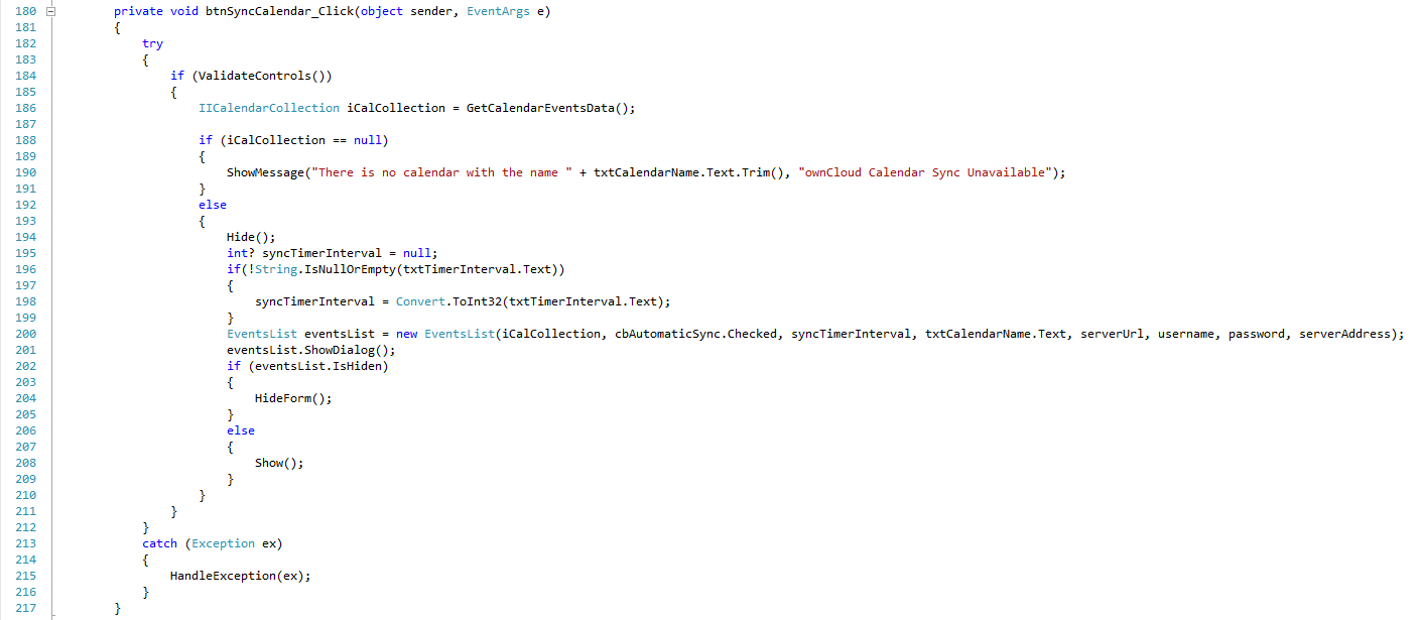
\includegraphics[scale=0.5]{slike/SyncCalendarMethod.png}
	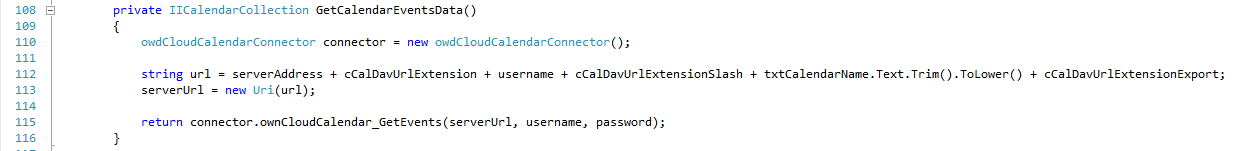
\includegraphics[scale=0.5]{slike/GetCalendarEventsDataMethod.png}
	\caption{Методе за синхронизацију догађаја са \textit{оwnCloud} календара}
	\label{fig:sync_calendar_method}
\end{figure}

\subsection{Аутоматска синхронизација догађаја}

Поред наведене функционалности за синхронизацију догађаја на захтев, омогућена је и функционалност аутоматске синхронизације догађаја. Уколико корисник жели да користи дату функционалност, потребно је да чекира опцију \textit{Automatic sync} на форми за синхронизацију догађаја (Слика \ref{fig:sync_calendar}). Када је опција \textit{Automatic sync} чекирана, податак \textit{Sync time interval} је обавезан. Дакле, након дефинисања наведених података, апликација ће аутоматски синхронизовати догађаје са одговарајућег календара у наведеном временском интервалу. Времески интервал се дефинише у минутима и одговарајућом валидацијом онемогућемо је да вредност овог податка буде било шта што није цео позитиван број.

\subsection{Преглед преузетих догађаја}
Када су сви обавезни подаци исправно унети, било да је у питању синхронизација догађаја на захтев, било да је у питању аутоматска синхронизација догађаја, кликом на дугме \textit{Sync now} (Слика \ref{fig:sync_calendar_personal}) прузимају се догађаји са одговарајућег календара и прикаже се форма са листом догађаја (Слика \ref{fig:events_list}):

\begin{figure}[H]
	\centering
	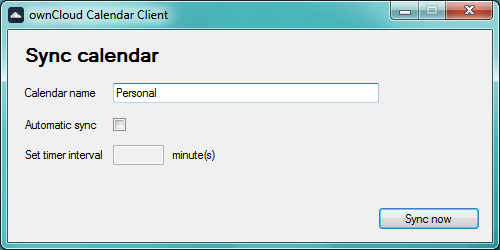
\includegraphics[scale=0.5]{slike/SyncCalendarPersonal.png}
	\caption{Синхронизација догађаја са \textit{оwnCloud} календара}
	\label{fig:sync_calendar_personal}
\end{figure}

\begin{figure}[H]
	\centering
	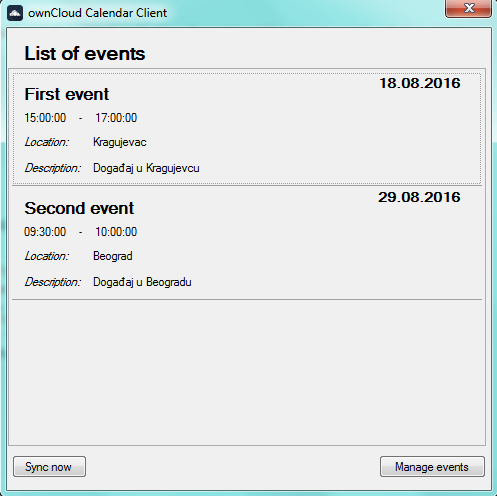
\includegraphics[scale=0.5]{slike/EventsList}
	\caption{Приказ преузетих догађаја}
	\label{fig:events_list}
\end{figure}

Са форме за Преглед преузетих догађаја (Слика \ref{fig:events_list}) корисник у сваком тренутку може поново да покрене синхронизацију догађаја (кликом на дугме \textit{Sync now}), без обзира на то да ли је функционалност аутоматске синхронизације изабрана или не. Корисник, такође, има могућност да са форме за Преглед преузетих догађаја  (Слика \ref{fig:events_list}), кликом на дугме \textit{Manage events} приступи календару на веб порталу \textit{оwnCloud} платформе (Слика \ref{fig:own_cloud_calendar})  и администрира (креира нове, ажурира постојеће, брише) догађаје.

\subsection{Приказ нотификација}

Поред описаних функционалности апликација има још једну, вероватно најзанимљивију функционалност, а то је приказ одговарајућих нотификација у вези са преузетим догађајима. Нотификације се приказују према унапред дефинисаним параметрима:
\begin{itemize}
	\item{први параметар (\textit{notificationMessageTimerInMinutes}) представља временски период (у минутима) којим се дефинише колико минута пре стартовања догађаја приказати одговарајућу нотификацију},
	\item{други параметар (\textit{notificationPingTimeInterval}) представља времески период (у милисекундама) којим се дефинише колико често ће се проверавати да ли је први параметар достигао дефинисану вредност}.	

\end{itemize}
Ови параметри су конфигурабилни и део су конфигурационог фајла:

\begin{figure}[H]
	\centering
	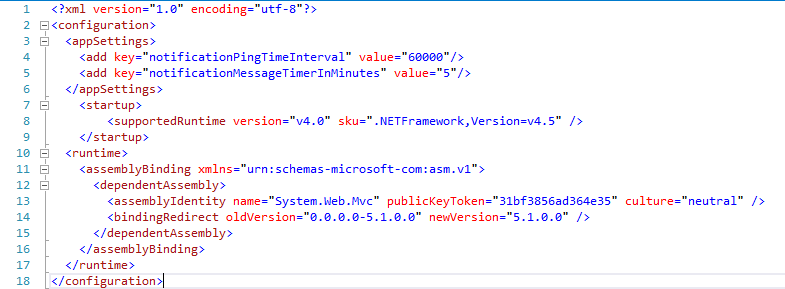
\includegraphics[scale=0.5]{slike/AppConfig.png}
	\caption{Конфигурациони фајлl}
	\label{fig:app_config}
\end{figure}

Дакле, у складу са дефинисаним вредностима наведених параметара, апликација сваког минута проверава да ли постоји догађај који ће стартовати за 5 минута и у случају да такав догађај постоји, кориснику се прикаже одговарајућа нотификација:

\begin{figure}[H]
	\centering
	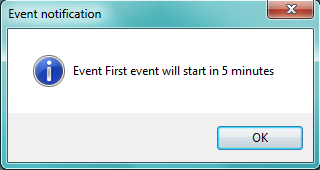
\includegraphics[scale=0.5]{slike/EventNotification.png}
	\caption{Приказ нотификације}
	\label{fig:event_notification}
\end{figure}

У наставку је приказана метода којом је дата функционалност имплементирана:

\begin{figure}[H]
	\centering
	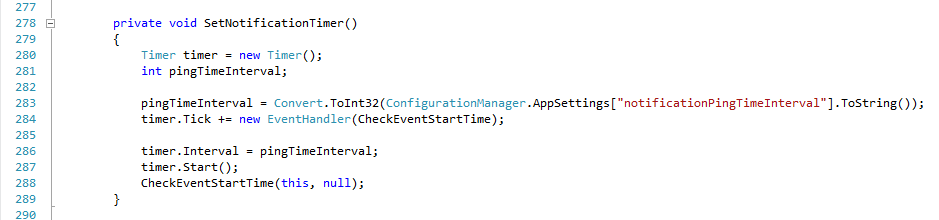
\includegraphics[scale=0.5]{slike/SetNotificationTimer.png}
	\caption{Метода за приказ нотификација}
	\label{fig:set_notification_timer}
\end{figure}

Поред функционалности описаних у претходним секцијама, споменућемо још нека свoјства апликације. Најпре, треба нагласити да је апликација \textit{Single instance}, односно у једном тренутку могуће је покренути само једну инстанцу апликације. У случају да корисник покуша да покрене више инстанци апликације, то му неће бити дозвоњено и приказаће се одговарајућа порука. 
Такође, требало би напоменути да се кликом на дугме \textit{Close} на форми за Приказ преузетих догађаја апликација не затвара, већ се само минимизације, тј. апликација је и даље покренута и иконица апликације налази се у таскбару (Слика \ref{fig:application_icon}):

\begin{figure}[H]
	\centering
	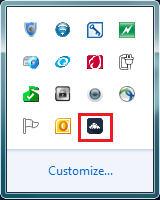
\includegraphics[scale=0.5]{slike/ApplicationIcon.png}
	\caption{Таскбар - приказ иконице}
	\label{fig:application_icon}
\end{figure}

Десни клик на иконицу у таскбару нуди следеће опције (Слика \ref{fig:icon_right_click}):
\begin{itemize}
	\item{отварање форме за приказ преузетих догађаја},
	\item{отварање форме за унос параметара синхронизације},
	\item{одјава са апликације и приказ форме за пријаву},
	\item{затварање апликације}.
\end{itemize}

\begin{figure}[H]
	\centering
	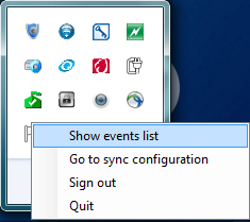
\includegraphics[scale=0.5]{slike/IconRightClick.png}
	\caption{Додатне опције}
	\label{fig:icon_right_click}
\end{figure}

\section{Идеје за даљи развој}

Иако је функционално исправна, постојећу верзију апликације треба посматрати само као полазни корак у развоју коначног производа. Актуелна верзија апликације има својеврсна ограничења условњена коришћеним API-има (нпр. немогућност синронизације више календара истовремено). Унапређења датих API-a или појава нових утицали би на то да се појави потреба за имплементацијом додатних функционалности. Са друге стране, постојећа верзија се такође може унапредити на више начина:
\begin{itemize}
	\item{побољшање корисничког интерфејса},
	\item{предефинисани прикази догађаја (за разлику од актуелног приказа свих догађаја)},
	\item{...}
\end{itemize}